\section{アプリケーション層}
アプリケーション層は,OSI参照モデルの第7層,またTCP/IP参照モデルでは第4層に位置するレイヤのことを指す.
このレイヤは,ネットワークを介したアプリケーション(ソフトウェア,プログラム)の通信プロトコルを定義している.
これらのアプリケーションに対して,透過的なネットワーク通信を実現するインタフェースを提供し,
ユーザアプリケーションによる情報のやり取りを容易にしている.
例えば,インターネット上においてデータ通信の要となっているのはHTTPとよばれるプロトコルである.
従って,普段Webブラウザでインターネット上のページを見るときは,そのページを提供しているWebサーバとの間で
HTTP通信を行っていることが多い.

アプリケーション層で定義されているプロトコルには,代表的なものとして,HTTPやDHCP,DNS,SMTP,Telnet,FTPが存在する.
この他にも切りがないほど数多くのプロトコルが定義されているが,
本節では,そのなかでも特にメジャーなプロトコルについて説明する.

\subsection{HTTP}
HTTP(HyperText Transfer Protocol)とは,インターネット上においてコンテンツ(HTML,テキスト,画像等)を
送信するための規定を定めたものである.
現在の主流なバージョンは,HTTP/1.1とHTTP/2.0である.近年は,HTTP/2.0の仕様が標準として定められたことにより,
続々とHTTP/2サーバが実装されており,今後の主流になると考えられる.
またHTTPでは,デフォルトでTCPの80番ポートを使用する.

HTTPは通信を暗号化しないため,仮に通信を盗聴された場合に内容が閲覧されたり,
通信内容を改ざんされる危険性がある.そのため,HTTPの通信をセキュアにしたHTTPSという規格も存在している.

\subsubsection{HTTP通信の流れ}
HTTPにおける典型的な通信の流れは,まずWebクライアント(通常はWebブラウザ)がWebサーバに存在するコンテンツに対して
HTTPリクエストを発行するところから始まる.
このとき,Webサーバ上にあるコンテンツは,URI(Uniform Resource Identifier)によって一意に識別される.
Webサーバ側はHTTPリクエストを受け取った後,それに対応するHTTPレスポンスをWebクライアントに返す.
HTTP通信は,実際にこのように単純な仕組みで成り立っている.実際の通信の流れを,図\ref{fig:httpflow}に示す.

この例では,Webブラウザを用いて\url{http://www.kansai-u.ac.jp/index.html}というURLにアクセスしようとしている.
Webブラウザは,\url{www.kansai-u.ac.jp}のWebサーバに対して,index.htmlというコンテンツを要求する
HTTPリクエストを送信する.そして,Webサーバ側はindex.htmlを含むHTTPレスポンスを返す.
最後にクライアント側では,レスポンス内容であるindex.htmlをWebブラウザ上に表示している.

\begin{figure}[htbp]
    \centering
    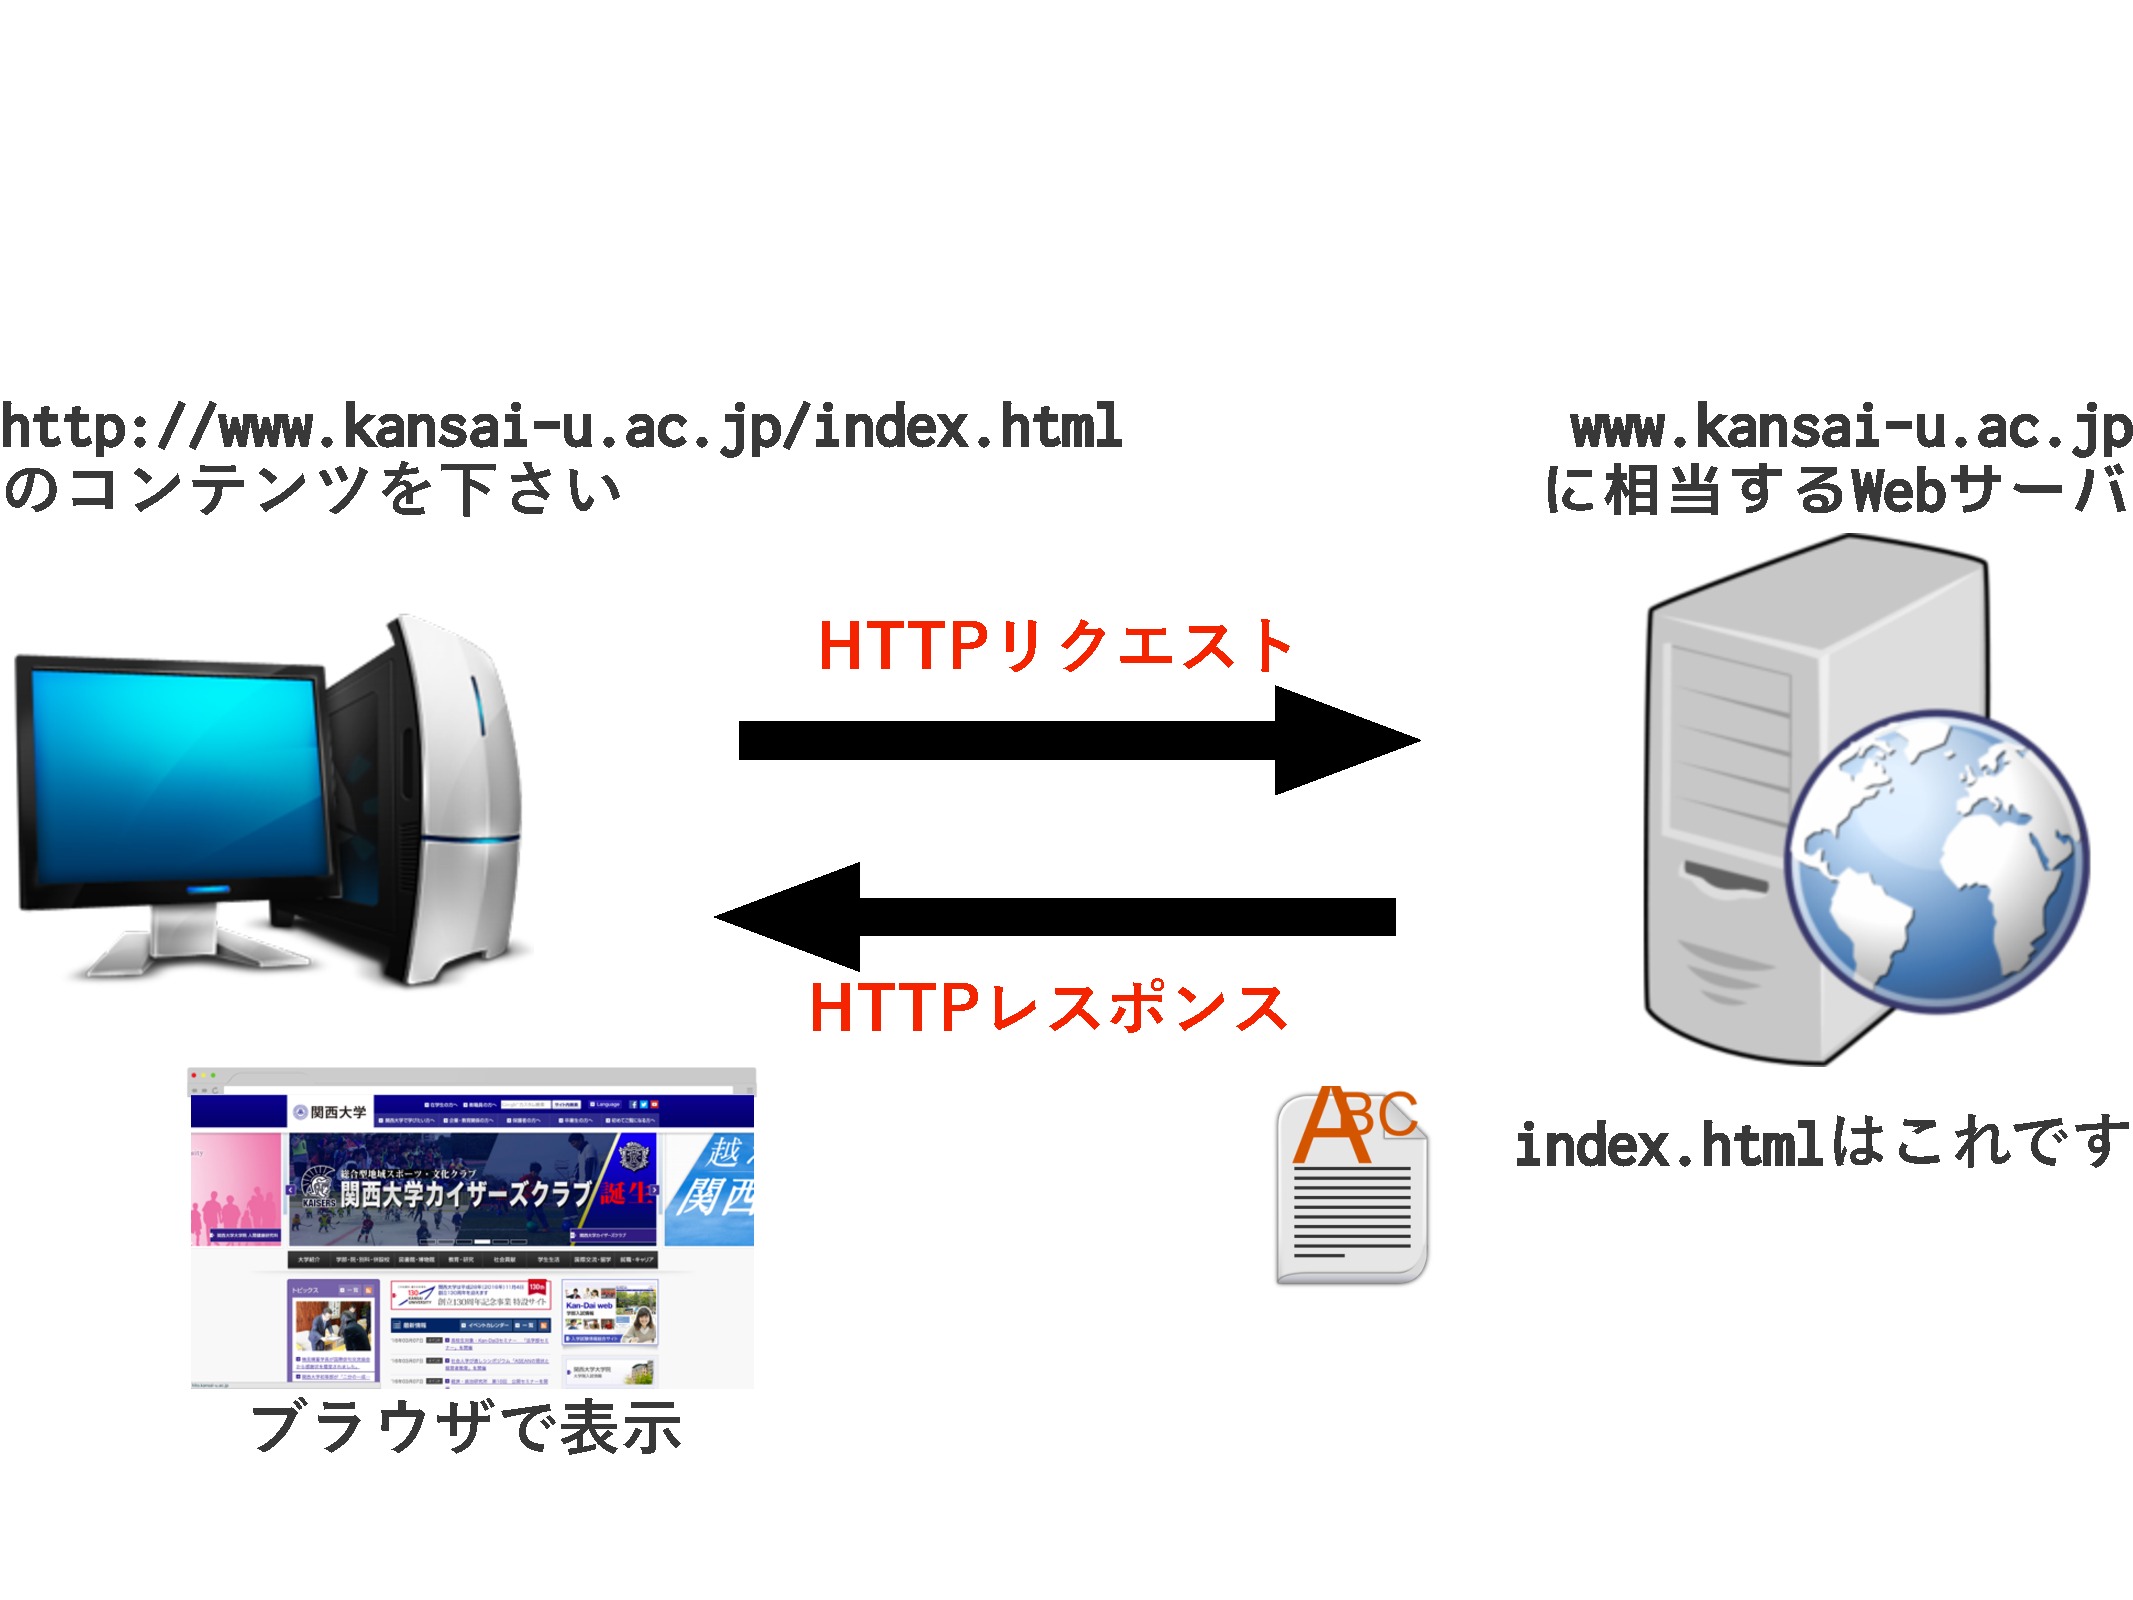
\includegraphics[width=0.9\hsize]{httpflow.pdf}
    \caption{HTTP通信の流れ}
    \label{fig:httpflow}
\end{figure}

また上記の例における通信をテキストベースで表現したものが,リスト\ref{list:httpreq}とリスト\ref{list:httpres}に当たる.
「/index.html」というURIに対して,「GET」というメソッドを用いて,
HTTP/1.1バージョンで通信をしているといった具合だ.HTTPメソッドについては,後述する.

\begin{lstlisting}[basicstyle=\ttfamily\small, numbers=none, frame=tlrb, caption=HTTPリクエスト, label=list:httpreq]
GET /index.html HTTP/1.1
Host: www.kansai-u.ac.jp
\end{lstlisting}

上述のリクエストに対するHTTPレスポンスが次のものになる.
\begin{lstlisting}[basicstyle=\ttfamily\small, numbers=none, frame=tlrb, caption=HTTPレスポンス, label=list:httpres]
HTTP/1.1 200 OK
Date: Wed, 09 Mar 2016 16:50:39 GMT
Server: Apache
Accept-Ranges: bytes
Content-Length: 30569
Connection: close
Content-Type: text/html
Content-Language: ja

<index.htmlのHTMLコード>
\end{lstlisting}

\subsubsection{HTTPヘッダ}
HTTPでは,リクエストとレスポンス双方の通信に,ヘッダと呼ばれるものを付けて通信を行う.
このヘッダを付けることによって,一つ一つの通信を詳細化することや区別すること,最適化することが可能となる.
表\ref{tab:reqheader}と表\ref{tab:resheader}に,主なHTTPヘッダとその用途を示す.
ここで挙げた以外にも様々なヘッダが用意されており,それらを用いることにより,効果的なHTTP通信を実現している.
例えば,HTTP通信を減らすためにブラウザにコンテンツをキャッシュしたいとき,
HTTPヘッダを使って,ある程度の操作が出来る.

\begin{table}[htbp]
    \centering
    \caption{HTTPリクエストヘッダ一覧}
    \label{tab:reqheader}
    \begin{tabular}{c|c} \hline
        ヘッダ & 用途 \\ \hline
        Host & リクエスト先のサーバ名を示す \\ \hline
        Cookie & クライアントの状態管理情報をサーバに送る \\ \hline
        Accept & クライアントの受け入れ可能コンテンツタイプを返す \\ \hline
        Authorization & クライアントの認証情報を返す \\ \hline
    \end{tabular}
\end{table}
\begin{table}[htbp]
    \centering
    \caption{HTTPレスポンスヘッダ一覧}
    \label{tab:resheader}
    \begin{tabular}{c|c} \hline
        ヘッダ & 用途 \\ \hline
        Server & Webサーバの情報を返す \\ \hline
        WWW-Authenticate & 認証領域名を示す固有値 \\ \hline
    \end{tabular}
\end{table}


\subsubsection{HTTPメソッド}
HTTPリクエストは,そのリクエストが何を意味しているかを示すために,メソッドと呼ばれる種類で分けられる.
主なメソッドとして,「GET」と「POST」が挙げられる.
通常,「GET」メソッドは,主にWebページ等のコンテンツを取得するときに使われ,
「POST」メソッドは,Webサーバにデータを送りたいときに使われる.
この他,「PUT」や「DELETE」,「HEAD」が存在する.
RESTful API等を考えない限り,現状変わった挙動はない.

\subsection{FTP}
FTPとは,File Transfer Protocolの略で,ネットワークを用いたファイル転送のためのプロトコルである.
主に,Web用のコンテンツファイル(HTMLファイルや画像等)をサーバ上にアップロードするときや,
フリーソフト等をクライアントがダウンロードしたいときなどに使われていた.
FTPは,プロトコル自体に暗号化の仕組みが存在しないため,HTTP同様に通信の盗聴が容易である.
セキュアな通信を確立するため,FTPに暗号化通信の仕組みを組み込んだFTPSや,後述するSSHという仕組みを用いて通信を暗号化するSFTPが存在する.

\subsection{SSH}
SSHとは,Secure Shellの略で,暗号化された通信上で,リモートコンピュータにログインするためのプロトコルである.
全ての通信は,ログインのためのパスワード情報等も含めて暗号化されているため,盗聴されていたとしても内容が漏洩する心配はない.
ログイン方法には,パスワードを使ったパスワード認証と公開鍵を用いた公開鍵認証があり,
認証情報をよりセキュアに管理するには公開鍵認証を使ったほうが良い.

SSHは,他のサービスとも一緒に使われることがあり,上述したFTPをSSH通信で実現するSFTPや,SFTPに似たものでリモートコンピュータ上に安全にファイルをコピーするためのscpというものが存在する.

